\chapter{پیاده‌سازی و نتایج}
\pagebreak
\section{مقدمه}
در فصل گذشته، معماری پیشنهادی، که مبتنی بر شبکه‌ی عصبی کانولوشنی و ترنسفورمر بود، به تفصیل معرفی گردید. برای بررسی عملکرد آن، مدل پیشنهادی پیاده‌سازی شده و نتایج آن با سایر مدل‌های مطرح در درک زبان طبیعی مقایسه گردید. در فصل پیش رو، تنظیمات و شرایط استفاده شده برای انجام آزمایش‌ها شرح داده می‌شود. سپس، نتایج پیاده سازی مدل پیشنهادی با سایر مدل‌های مطرح مقایسه می‌گردد. در انتهای فصل، به تحلیل میزان اثربخشی هر بخش از مدل پیشنهادی، در نتیجه‌ای که به دست آمده پرداخته می‌شود. 

\section{مجموعه داده}
به منظور بررسی عملکرد مدل پیشنهادی، آزمایش‌های این فصل بر روی دو مجموعه داده‌ی شناخته شده‌ی \lr{ATIS} و \lr{SNIPS} انجام می‌شود. این دو مجموعه داده، در میان مدل‌های درک زبان طبیعی به عنوان یک چالش، برای سنجش عادلانه‌ی عملکرد مدل‌ها و مقایسه‌ی نتایج با کارهای پیشین استفاده می‌شوند. برچسب‌های پر کردن جای خالی، گاهی دارای مفهوم هستند، اما مرسوم است برای آن‌ها، تعبیه‌ی مبتنی بر واژه ایجاد نشود. برای استفاده از این مجموعه داده، مدل بر روی مجموعه داده‌ی آموزشی، آموزش داده شده و ابر پارامترها بر روی مجموعه داده‌ی ارزیابی تنظیم شدند. سپس، نتایج پایانی روی مجموعه‌ی تست گزارش شد. برخی از برچسب‌های هدف و اهداف کاربر، در زمان آموزش مشاهده نشده‌اند. در چنین مواردی، کلاس \lr{''Unknown''} به آن‌ها اختصاص داده شد. در ادامه، این دو مجموعه داده معرفی می‌شوند.
\subsection{\lr{ATIS}}
\lr{ATIS}\LTRfootnote{Airline Travel Information Systems} 
که به صورت گسترده برای سنجش عملکرد مدل‌های درک زبان طبیعی مورد استفاده قرار گرفته است \cite{5700816}، یک مجموعه داده در مورد انسان‌هایی است که از سیستم‌های خودکار استعلام سفر هواپیمایی\LTRfootnote{Automated Airline Travel Inquiry Systems} سؤال مورد نظر خود را می‌پرسند \cite{atis:hemphill1990}. زمینه‌های تحت پوشش این مجموعه داده شامل پرسش در مورد پروازها، هزینه‌ی پرواز، خطوط هواپیمایی، شهرها، فرودگاه‌ها و خدمات زمینی می‌شود. این مجموعه داده شامل ۴۴۷۸ نمونه برای آموزش، ۵۰۰ نمونه برای ارزیابی و ۸۹۳ نمونه برای آزمایش می‌باشد. \lr{ATIS} دارای ۱۲۷ نوع برچسب یکتا، و همچنین ۲۱ هدف کاربر یکتا است. توزیع این نمونه‌ها به صورت نامتوازن بوده و میانگین طول جملات آن، ۱۱ واژه است.
\subsection{\lr{SNIPS}}
\lr{SNIPS} 
 یک مجموعه داده‌ی تولید شده از دستیار شخصی دیجیتال \lr{SNIPS} است، که دارای ۱۳۰۸۴ نمونه برای آموزش، ۷۰۰ نمونه برای ارزیابی و 700 نمونه برای آزمایش است \cite{snips:coucke2018}. همچنین، این مجموعه داده دارای ۷ نوع هدف یکتا و ۷۲ برچسب یکتا می‌باشد. در تضاد با \lr{ATIS}، مجموعه داده‌ی \lr{SNIPS} شامل پرسش درباره‌ی آب و هوا، رستوران‌ها، سرگرمی و غیره بوده  و دایره‌ی واژگانی آن گسترده‌تر است. توزیع نمونه‌های این مجموعه داده به صورت متوازن بوده و میانگین تعداد واژه‌ها در جمله، برابر ۹ است.
\section{معیارهای ارزیابی}
بعد از آشنایی با مجموعه داده‌های مورد استفاده، معیارهایی که در زمینه‌ی درک زبان طبیعی برای سنجش عملکرد مدل‌ها استفاده شده‌اند، معرفی می‌شوند. برای سنجش عملکرد در وظیفه‌ی پر کردن جای خالی، امتیاز \lr{micro f1}، و برای سنجش عملکرد تشخیص هدف، معیار دقت\LTRfootnote{Accuracy} استفاده می‌گردد.
\subsection{امتیاز \lr{f1} برای پر کردن جای خالی}
امتیاز \lr{f1} معیاری است که برای هر کلاس محاسبه می‌شود؛ به این معنی که اگر مقصود محاسبه‌ی امتیاز کلی \lr{f1} را برای مجموعه داده‌ای با بیش از یک کلاس باشد، باید به نحوی امتیازات به دست آمده جمع شود. امتیاز \lr{f1} به دو شیوه‌ی \lr{micro f1} و \lr{macro f1} جمع می‌شود. در شیوه‌ی \lr{macro f1}، ابتدا درستی\LTRfootnote{Precision} و به یاد آوری\LTRfootnote{Recall} هر کلاس محاسبه شده و سپس، میان درستی هر کلاس و به یاد آوری کلاس‌ها میانگین گرفته می‌شود. اما در مقابل، در شیوه‌ی \lr{micro f1} که در معادله‌ی \ref{Eq:microf1} تعریف شده، به جای میانگین گیری میان دقت و به یاد آوری، امتیاز \lr{f1} با استفاده از تعداد کل مثبت واقعی $TP$، مثبت کاذب $FP$ و منفی کاذب $FN$ حساب می‌شود. در این معادله، $c$ بیانگر تعداد کلاس‌ها است.
\begin{equation}
	Micro\,f1 = \frac{\sum^{c}TP}{\sum^{c}TP+\frac{1}{2}(\sum^{c}FP+\sum^{c}FN)}
	\label{Eq:microf1}
\end{equation}


در وظیفه‌ی پر کردن جای خالی، از امتیاز \lr{micro f1} استفاده شده است. علت استفاده از معیار \lr{micro} به جای \lr{macro}، در وظیفه‌ی پر کردن جای خالی، این است میزان توانایی حدس زدن یک کلاس برای این وظیفه کم اهمیت است؛ زیرا با وجود نامتوازن بودن برچسب‌ها، درصورت انتخاب اشتباه کلاس پر استفاده‌ی \lr{O} در مجموع داده‌ها، خروجی سیستم گفت‌وگو تحت تاثیر قرار می‌گیرد. به این معنا که در تشخیص اشتباه کلاس پر مثال \lr{O} و یک کلاس کم مثال، تفاوتی نیست. از این جهت، تمامی کلاس‌ها برای این وظیفه از اهمیت یکسان برخوردارند.


\subsection{دقت برای تشخیص هدف}
برای سنجش وظیفه‌ی تشخیص هدف، از معیار دقت استفاده می‌شود. معیار دقت، حاصل تقسیم تعداد نمونه‌های صحیح پیش‌بینی شده، بر تعداد کل پیش‌بینی ها است.
\section{تنظیمات آزمایش}\noindent
ابر پارامترها\LTRfootnote{Hyper-parameters} نقش اساسی در عملکرد یک مدل شبکه عصبی دارند. از آن‌جا که هر جزء \lr{CTran} از انواع شبکه‌های عصبی متفاوت استفاده می‌کند، از نرخ‌های یادگیری متفاوت $\alpha$ با بهینه ساز \lr{AdamW} \cite{adamw:Loshchilov} برای هر لایه استفاده شد. \lr{CTran} با بهره بری از زمان‌بند \lr{StepLR}، نرخ یادگیری پارامترها در هر دور آموزش، با ضریب $\gamma$ کاهش می‌یابد. همچنین، حذف تصادفی\LTRfootnote{dropout} روی لایه‌ها اعمال می‌شود، تا میزان بیش‌برازش\LTRfootnote{Overfitting} را کاهش دهد \cite{dropout:Srivastava}. همچنین مشاهده شد که استفاده از برش گرادیان\LTRfootnote{Gradient Clipping} با مقدار 0/5 به عملکرد نهائی مدل کمک می‌کند \cite{clipping:mikolov}. جدول \ref{Tab:rates}، $\alpha$، $\gamma$ و $\rho$ را برای هر لایه نشان می‌دهد. همچنین اندازه‌ی دسته\LTRfootnote{Batch-Size} در هر دو مجموعه داده برابر 16 می‌باشد.


برای اندازه‌ی هسته،اندازه‌های 1، 2، 3، [1،3]، [1،3،5]، [2،3،5]، و [1،2،3،5] امتحان شد، که در آن براکت‌ها نشان‌دهنده‌ی استفاده‌ی چند اندازه‌ی هسته به صورت همزمان است. تعداد هسته‌ها به صورت تجمعی همیشه برابر 512 می‌باشد و تعداد هسته‌ها به طور مساوی بین هسته‌های مختلف پخش می‌شود.
\begin{table*}[ht]
	\input{Tables/rates.txt}
	\caption[ابر پارامتر‌های استفاده شده در فاز آموزش]{
		ابر پارامتر‌های استفاده شده در فاز آموزش. در این جدول، نرخ یادگیری $\alpha$، نرخ زمان بند $\lambda$ و احتمال حذف تصادفی $\rho$ استفاده شده برای هر لایه در زمان آموزش مدل پیشنهادی هستند.
	}
	\label{Tab:rates}
\end{table*}


روش‌های گوناگونی برای توقف فرایند آموزش وجود دارد. از میان این روش‌ها می‌توان به مکانیزم توقف درصورت عدم رشد، توقف زودرس و توقف با تعداد دور مشخص اشاره کرد. تمامی مدل‌هایی که در فصل ۳ از آن‌ها نام برده شد، از شیوه‌ی توقف با دور مشخص استفاده کردند. در مدل پیشنهادی نیز، از این مکانیزم برای آموزش مدل استفاده گردید. بدین منظور، برای هر آزمایش، مدل برای ۵۰ دور روی مجموعه داده آموزش داده شد و در هر دور از آموزش، نتیجه‌ی آن گزارش گردید. زمانی که دو وظیفه‌ی پر کردن جای خالی و تشخیص هدف، همزمان حداکثر شوند، به عنوان حداکثر دقت مدل در نظر گرفته می‌شوند. برای اطمینان از صحت هر آزمایش، هرکدام از آن‌ها 10 بار اجرا شدند، که هر یک شامل 50 دور آموزش بود. در نهایت، برای گزارش نتیجه‌ی آزمایش، مقدار میانه، از میان ۱۰ بار انجام آزمایش، گزارش شد.
%Table 2 of the paper


\section{نتایج و آنالیز}
\begin{table*}[ht]
		\input{Tables/final_atis.txt}
	\caption[مقایسه میان مدل پیشنهادی و سایر مدل‌های شناخته شده بر روی مجموعه داده‌ی \lr{ATIS}]{
		مقایسه میان مدل پیشنهادی و سایر مدل‌های شناخته شده بر روی مجموعه داده‌ی \lr{ATIS}. علامت $\beta$ نمایانگر استفاده‌ی برت در طراحی مدل است. مقادیر همگی به درصد هستند.
	}
	\label{Tab:final_atis}
\end{table*}
زمانی که مدل‌ها به دقت ۱۰۰ درصد نزدیک می‌شوند، پیشرفت‌ها کوچک‌تر شده و سخت‌تر به دست می‌آیند. جدول \ref{Tab:final_atis}، نتایج مدل پیشنهادی در این پایان‌نامه را، با مدل‌های شناخته شده‌ی فعلی، که بالاترین عملکرد را در مجموعه داده‌ی \lr{ATIS} دارند، مقایسه می‌کند. مدل \lr{CTran+BERT\textsubscript{large}} در وظیفه‌ی پر کردن جای خالی و بر روی مجموعه‌داده‌ی \lr{ATIS}، از همه‌ی مدل‌های موجود عملکرد بهتری نشان می‌دهد. مدل پیشنهادی ما، نسبت به بالاترین عملکرد در گذشته، ۰‍/۶۴ درصد بهبود را نشان می‌دهد. همچنین، مدل پیشنهادی برای وظیفه‌ی تشخیص هدف، نسبت به مدل پایه  که مشابه این پایان‌نامه، از ساختار کانولوشن-توالی پنجره ویژگی استفاده کرده است، 0‍/9 درصد بهبود را نشان می‌دهد.
\begin{table*}[ht]
	\input{Tables/final_snips.txt}
	\caption[مقایسه‌ی مدل پیشنهادی و سایر مدل‌های شناخته شده بر روی مجموعه داده‌ی \lr{SNIPS}]{
		مقایسه‌ی مدل پیشنهادی و سایر مدل‌های شناخته شده بر روی مجموعه داده‌ی \lr{SNIPS}. علامت $\beta$ نمایانگر استفاده‌ی برت در طراحی مدل است. مقادیر همگی به درصد هستند.
	}
	\label{Tab:final_snips}
\end{table*}


برای سنجیدن صحت برتری مدل \lr{CTran} نسبت به کارهای پیشین، عملکرد آن روی مجموعه داده‌ی \lr{SNIPS} نیز سنجیده‌شد. جدول \ref{Tab:final_snips} دقت مدل‌های شناخته شده را با \lr{CTran} مقایسه می‌کند. برای مجموعه داده‌ی \lr{SNIPS}، \lr{f1} مدل پیشنهادی در پر کردن جای خالی، نسبت به بهترین مدل موجود، ۱ درصد افزایش دارد. اگرچه عملکرد \lr{CTran} در وظیفه‌ی تشخیص هدف، نسبت به اکثر مدل‌های پیشین برتری دارد، اما از بهترین نتیجه‌ی موجود پیشی نمی‌گیرد و رتبه‌ی دوم را در این وظیفه به خود اختصاص می‌دهد.
در زیر بخش‌های بعدی، بررسی می‌شود که چقدر هر ایده، \lr{CTran} را بهبود داده است.
\subsection{اثر لایه کانولوشن با رمزنگار ترنسفورمر}
از آن‌جا که در کارهای گذشته، از شبکه‌ی عصبی کانولوشنی برای رفع نقص شبکه عصبی بازگشتی استفاده می‌کرده‌اند، ممکن است بهره‌مندی از رمزنگار ترنسفورمر باعث کاهش اهمیت شبکه‌ی کانولوشنی شود. هدف از استفاده از معماری کانولوشن-توالی ویژگی پنجره با رمزنگار ترنسفورمر، آمیخته کردن تعبیه‌ی نشانه‌های مجاور در یکدیگر می‌باشد. جدول \ref{Tab:cnn_wfs_te}، عملکرد پشته‌ی رمزنگار ترنسفورمر تنها را، در مقابل معماری رمزنگار \lr{CTran} می‌سنجد. همانطور که مشهود است، برای هر دو مجموعه داده‌ی \lr{ATIS} و \lr{SNIPS}، هر دو معیار تشخیص هدف و پرکردن جای خالی با استفاده از معماری پیشنهادی، افزایش یافته است. این نتایج، سودمندی فرایند آمیختگی را تایید می‌کند. همچنین، این نتیجه نشان می‌دهد که با وجود توانمندی ترنسفورمر در درک دوطرفه‌ی معنای جمله، می‌توان با اضافه کردن معنای واژه‌های اطراف، به تعبیه‌ای غنی‌تر دست یافت.
\begin{table*}[ht]
		\input{Tables/cnn_wfs_te.txt}
	\caption[مقایسه‌ی عملکرد رمزنگار ترنسفورمر، با ساختار کانولوشن-توالی ویژگی پنجره-پشته‌ی رمزنگار ترنسفورمر]{
		مقایسه‌ی عملکرد رمزنگار ترنسفورمر تنها، با ساختار کانولوشن-توالی ویژگی پنجره-پشته‌ی رمزنگار ترنسفورمر. آزمایش‌ها با مدل زبانی $BERT_{base}$ صورت گرفته است. مقادیر همگی به درصد هستند.
	}
\label{Tab:cnn_wfs_te}
\end{table*}
\subsection{اندازه‌ی هسته}
اندازه‌ی هسته، بازه‌ای را که نشانه‌های در آن، با یکدیگر آمیخته می‌شوند را مشخص می‌کند. همچنین، می‌توان اندازه‌ی هسته را در کانولوشن، با \lr{n-gram}ها مقایسه کرد؛ به نحوی که اندازه‌ی هسته ۲ مانند \lr{bi-gram} است. تاکنون، اندازه هسته‌ی ۱ برای مدل‌های درک زبان طبیعی که مانند \lr{CTran} از شبکه‌ی کانولوشنی بهره می‌برند، استفاده نشده است. \lr{CTran} از اندازه‌ی ۱ برای حفظ صریح تعبیه‌ی نشانه استفاده می‌کند. همچنین، استفاده از اندازه‌ی ۱، باعث شده ابعاد تعبیه‌ی نشانه به اندازه‌ی سایر اندازه هسته‌ها شود. این امر سبب می‌شود که ضمن حفظ تعبیه‌ی صریح نشانه، تعبیه‌ی آمیخته با نشانه‌های همسایه نیز به آن اضافه شود. جدول \ref{Tab:cnn_kernelsize}، اثر اندازه‌های مختلف هسته را بر روی عملکرد \lr{CTran} نشان می‌دهد. در میان هسته‌های تک سایزی، ۱ از سایر موارد برای وظیفه‌ی پر کردن جای خالی عملکرد بهتری نشان داد. علت این امر، این است که اندازه‌ی هسته‌ی ۱، به نوعی مشابه \lr{1-gram} است، که این با رابطه‌ی یک به یک ورودی به برچسب خروجی تداخل ندارد. در همین راستا، مقایسه‌ی [2,3,5] و [1,2,3,5]، گفتار قبلی این پاراگراف را تایید می‌کند. بر مبنای این نتایج، می‌توان نتیجه گرفت که استفاده‌ی همزمان از چند اندازه‌ی هسته بهتر از هسته‌ی تک سایز است. در پایان، اندازه هسته‌ی [1,2,3,5] بهترین عملکرد را در هر دو وظیفه تشخیص هدف و پر کردن جای خالی دارد.
%Table 6 of the paper
\begin{table*}[ht]
		\input{Tables/cnn_kernelsize.txt}
	\caption[عملکرد مدل با اندازه هسته‌های متفاوت در لایه‌ی کانولوشنی]{
		عملکرد مدل با اندازه هسته‌های متفاوت در لایه‌ی کانولوشنی. براکت نشان دهنده‌ی استفاده از چند اندازه‌ی هسته به صورت همزمان است. مقادیر همگی به درصد هستند.
	}
\label{Tab:cnn_kernelsize}
\end{table*}

\subsection{ترازی رمزگشای ترنسفورمر}
رمزگشای ترنسفورمر اصلی، از هیچ ماسکی به جز ماسک‌های پد در بخش توجه متقابل استفاده نمی‌کند؛ به این معنی که در تولید هر نشانه هدف، بردار کلید تبدیل شده از تمام موقعیت‌های حافظه، در محاسبه توجه متقابل استفاده می‌شود. در مقابل، در رمزگشای ترنسفورمر تراز شده، تنها کلید تولید شده از زمینه مربوط به هر نشانه‌ی متناظر بر خروجی، روی توجه متقابل تأثیر می‌گذارد. به منظور تایید اثربخشی تراز پیشنهادی، رمزنگار \lr{CTran} با یک رمزگشای ترنسفورمر معمولی و در آزمایشی دیگر با یک \lr{LSTM} تراز شده با مکانیسم توجه که توسط \cite{Wang:18} ارائه داده شده است، ترکیب شد. در جدول \ref{Tab:notaligned}، \lr{f1} پر کردن جای خالی را از در هر سه مدل توصیف شده، مقایسه می‌کند، که در آن تراز پیشنهادی به طور متوسط 0‍/‍9 درصد بهبود را نسبت به رمزگشای ترنسفورمر معمولی نشان می‌دهد. علاوه بر این، مقایسه رمزگشای ترنسفورمر تراز شده‌ی پیشنهادی با رمزگشای \cite{Wang:18} در وظیفه‌ی پر کردن جای خالی 0‍/‍1 درصد بهبود را نشان می‌دهد. این امر، بیانگر این است که به طور کلی، معماری رمزگشای ترنسفورمر تراز شده، معماری بهتری برای وظیفه‌ی پر کردن جای خالی است.
%Table 7 of the paper
\begin{table*}[ht]
		\input{Tables/notaligned.txt}
	\caption[تاثیر ترازی رمزگشای ترنسفورمر بر روی مدل پیشنهادی]{
		تاثیر ترازی رمزگشای ترنسفورمر بر روی مدل پیشنهادی. اعداد نمایانگر میزان امتیاز \lr{f1} در وظیفه‌ی پر کردن جای خالی است. آزمایش‌ها با مدل زبانی $BERT_{base}$ صورت گرفته است. مقادیر همگی به درصد هستند.
	}
\label{Tab:notaligned}
\end{table*}

\subsection{شیوه‌ی استفاده از مدل زبانی در معماری مدل}
جدول \ref{Tab:strategy}، دو استراتژی مدل زبانی به عنوان رمزنگار و مدل زبانی به عنوان تعبیه‌ی واژه را با هم مقایسه می‌کند. در حالت اول، مدل زبانی به عنوان رمزنگار در معماری قرار گرفته، و برای رمزگشا، از رمزگشای پیشنهادی \lr{CTran} استفاده شده است. در مورد دوم، مدل زبانی نقش تعبیه‌گر واژه‌ها را دارد و تعبیه‌های تولید شده توسط مدل زبانی وارد رمزنگار \lr{CTran} می‌شود. \\
بر روی هر استراتژی، دو مدل زبانی برت و المو آزمایش گردید. بر اساس نتایج ما، استفاده از المو به عنوان رمزنگار، همراه با رمزگشای \lr{CTran}، از پیشرفته‌ترین مدل پر کردن جای خالی در \lr{ATIS} پیشی گرفته است. همچنین، هنگامی که المو تنها نقش تعبیه‌گر واژه‌ها را دارد، عملکرد مدل حتی از حالت قبلی نیز بهتر می‌شود و در هر دو وظیفه‌ی تشخیص هدف و پر کردن جای خالی، افزایش امتیاز مشاهده شد.


در مجموعه داده‌ی \lr{SNIPS}، استفاده از \lr{BERT\textsubscript{base}} به عنوان تعبیه‌ی واژه، عملکرد بهتری را در مقایسه با \lr{BERT\textsubscript{base}} به عنوان رمزنگار نشان می‌دهد. در مقابل، مدل زبانی به عنوان تعبیه‌ی واژه در \lr{ATIS} عملکرد خوبی نشان نداد و در نتیجه باعث بهبود نتایج نشد. علت این امر ممکن است کوچک بودن دایره‌ی واژگانی و همچنین تعداد کمتر مثال‌های آموزشی مجموعه‌ داده‌ی \lr{ATIS} باشد. از این رو، داشتن لایه‌های شبکه اضافی می‌تواند باعث بیش برازش مدل شود.
برای \lr{BERT\textsubscript{large}}، مدل زبانی به عنوان جاسازی کلمه، در هر دو مجموعه داده عملکرد خوبی داشت. علاوه بر این، معماری پیشنهادی با \lr{BERT\textsubscript{large}} به حداکثر کارایی دست یافت. اگرچه نتایج نشان می‌دهد که معماری پیشنهادی، بهترین عملکرد را نشان می‌دهد، اما بار محاسباتی بیشتری دارد. آزمایش‌های این بخش، نشان می‌دهد که برت در تمامی موارد، در قیاس با المو بهتر عمل می‌کند؛ اما المو می‌تواند برای مجموعه داده‌هایی که دامنه‌ی واژگانی محدودی دارند، با دقت عملکرد تقریباً مشابهی استفاده شود. این درحالی است که المو پیچیدگی محاسباتی و زمان آموزش کمتری دارد. علت وقوع این امر در این مورد، این است که مجموعه داده‌های هدف محور واژگان متنوعی ندارند؛ بنابراین حضور یک مدل زبانی پیش آموز شده را کمتر معنادار می‌کند. همچنین در آزمایش‌های صورت گرفته،  \lr{BERT\textsubscript{base}} و \lr{BERT\textsubscript{large}} برای کار تشخیص هدف مزیتی نسبت به یکدیگر ندارند. اما تفاوت آن‌ها در پر کردن جای خالی مشخص می‌شود، به نحوی که \lr{BERT\textsubscript{large}} نسبت به \lr{BERT\textsubscript{base}} برای همه مجموعه داده‌ها برتری خود را نشان می‌دهد.

%Table 8 of the paper
\begin{table*}[ht]
		\input{Tables/strategy.txt}
	\caption[دو استراتژی آزمایش شده برای پیدا کردن طرح مناسب برای معماری]{
		دو استراتژی آزمایش شده برای پیدا کردن طرح مناسب برای معماری.  از امتیاز \lr{F1} برای پر کردن جای خالی و معیار دقت برای تشخیص هدف استفاده گردید. مقادیر همگی به درصد هستند.
	}
\label{Tab:strategy}
\end{table*}

\section{هزینه‌ی محاسبات}
بار محاسباتی انجام تعبیه‌ی اضافی بعد از مدل زبانی، یک نگرانی به جا می‌باشد؛ زیرا در این استراتژی، پارامترهای بیشتری در شبکه تعریف می‌شوند. با توجه به اینکه از یک \lr{Nvidia RTX 3080} ۱۰ گیگابایتی برای محاسبات خود استفاده شد، جدول \ref{Tab:train_time} زمان آموزش را قبل و بعد از رمزنگار اضافی نشان می‌دهد. محاسبات نشان می‌دهد که بین 6 تا ۱۱ درصد زمان اضافی برای همگرایی مدل مورد نیاز است. برای این محاسبه، هر مدل را 10 بار، برای 10 دور آموزشی اجرا نموده و مقدار میانه گزارش شد.
\begin{table*}[ht]
		\input{Tables/train_time.txt}
	\caption[زمان اضافه شده به فرایند آموزش، با توجه به نقش مدل زبانی در معماری مدل]{
		زمان اضافه شده به فرایند آموزش، با توجه به نقش مدل زبانی در معماری مدل. مقدار زمانی اضافه، ناشی از حاصل استفاده از معماری کانولوشن-توالی ویژگی پنجره-ترنسفورمر است. مقادیر درون جدول نشان دهنده‌ی زمانی است برای یک دور آموزش مدل روی مجموعه داده‌ی مربوطه لازم است. واحد شمارش مقادیر، ثانیه است. مقادیر درون پرانتز نشانگر درصد افزایش زمان است.
	}
	\label{Tab:train_time}
\end{table*}
جدول \ref{Tab:inference_time}، زمان استنتاج مدل را نشان می‌دهد. برای این آزمایش، مدل 10 بار برای 200 نمونه و بدون دسته کردن ورودی اجرا و مقادیر میانگین گزارش شده است. اگرچه افزایش زمان تمرین محسوس بود اما افزایش زمان استنتاج بسیار ناچیز و تقریباً هم مقیاس با افزایش دقت مدل بود. با مقایسه قبل و بعد از استفاده از رمزنگار اضافی، بین ۱ تا ۱/‍‍۵ درصد تاخیر اضافی در استنتاج مشاهده می‌شود. این  افزایش در زمان آموزش و استنتاج قابل پیش‌بینی بود، زیرا معقول است که مدلی با پارامترهای بیشتر تاخیر اضافی داشته باشد.
\begin{table*}[ht]
		\input{Tables/inference_time.txt}	
	\caption[مقایسه‌ی زمان استنتاج مدل، با توجه به نقش مدل زبانی در معماری مدل]{
		مقایسه‌ی زمان استنتاج مدل، با توجه به نقش مدل زبانی در معماری مدل. مقادیر نشان دهنده‌ی تعداد میلی ثانیه‌ای است که برای استنتاج یک جمله‌ی ورودی لازم است. مقدار درون پرانتز نشان دهنده‌ی درصد افزایش است.
	}
\label{Tab:inference_time}
\end{table*}

\section{بررسی شیب آموزش}
\begin{figure}[!htb]
	\centering
	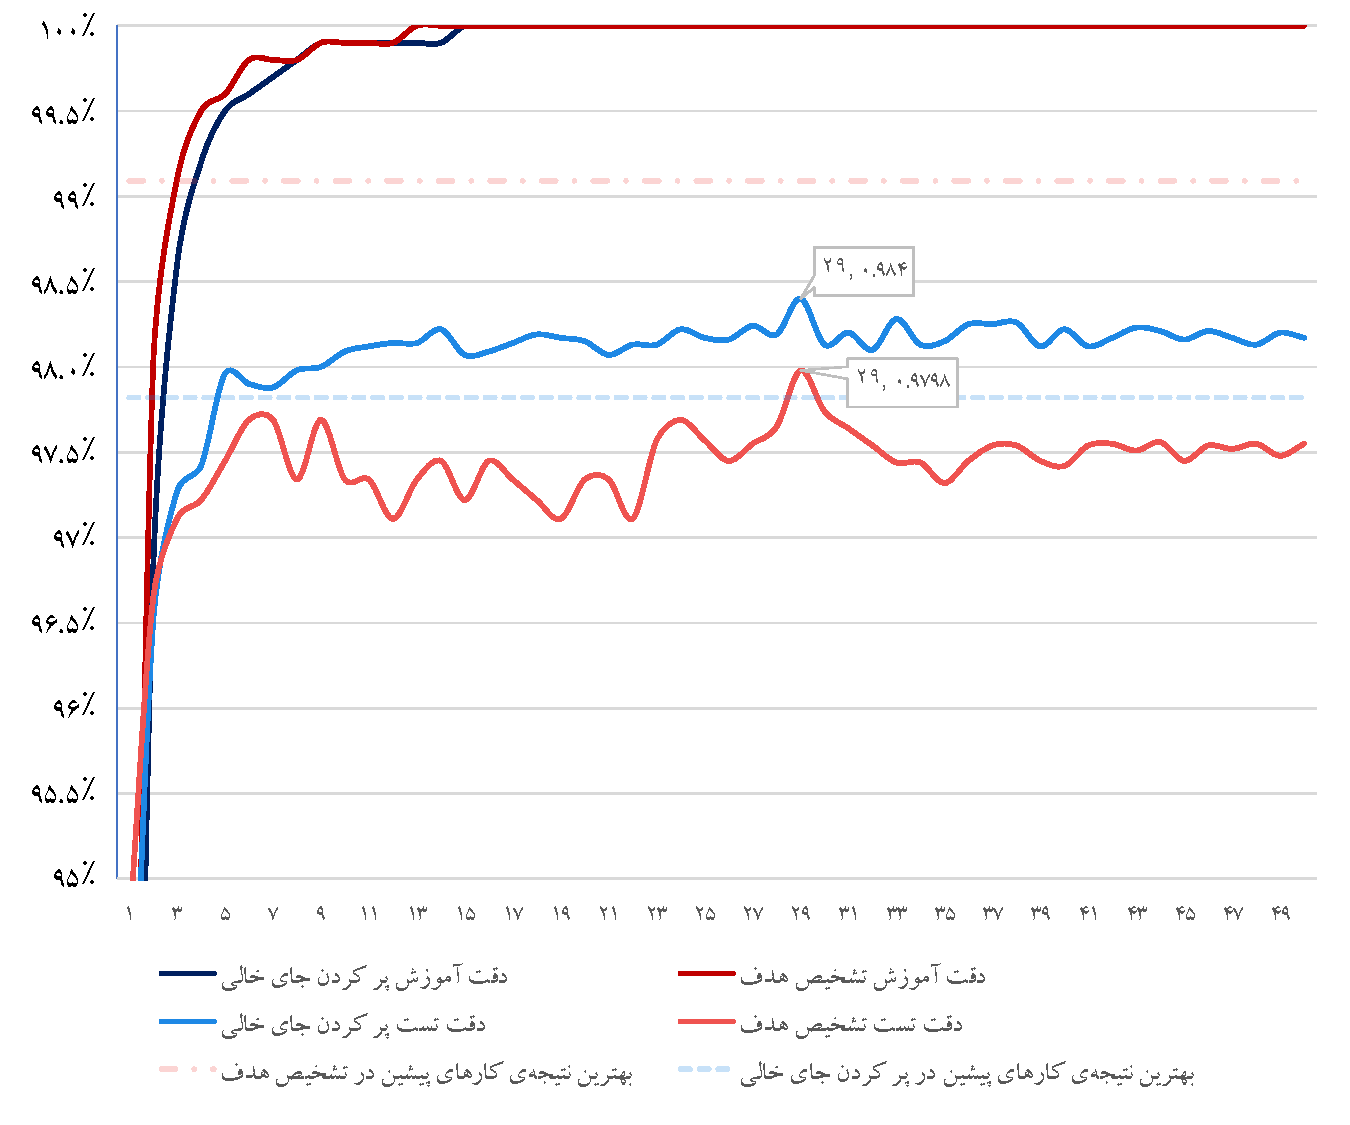
\includegraphics[scale=0.65]{Figures/atis_training_journey.pdf}
	\caption{شیب آموزش مدل پیشنهادی بر روی مجموعه داده‌ی \lr{ATIS}.}
	\label{Fig:atis_journey}
\end{figure}
شکل \ref{Fig:atis_journey} شیب آموزش مدل پیشنهادی به همراه $BERT_{large}$ را بر روی مجموعه داده‌ی \lr{ATIS} نشان می‌دهد. در راستای تحلیل وظیفه‌ی پر کردن جای خالی، در طول شیب آموزش مشاهده می‌شود که مدل در بازه‌ی دور ۱ تا ۱۰، دارای یک حداکثر محلی است. مدل در همین بازه نیز از کارهای پیشین سبقت می‌گیرد. برخی از کار‌های پیشین محدودیت ۱۰ دور را بر روی آموزش مدل اعمال کردند. در طول آزمایش‌ها مشاهده شد که مدل پس از اینکه در طول ۱۰ دور اول، مدل به حداکثر محلی رسیده و سپس رشد آن متوقف شده و گاهی کاهش می‌یابد. در این بازه، مدل شروع به حداکثر برازش خود رسیده و دقت مدل روی مجموعه‌ی آموزشی، به ۱۰۰درصد رسیده است. محدودیت تعداد دور آموزشی روی ۵۰ دور تنظیم شد. از این رو، پس از ۱۰ دور آموزش، مشاهده می‌شود که دقت مدل ثابت بوده و گاهی کاهش می‌یابد؛ اما در ادامه و در دور ۲۹-ام، حداکثر سراسری اتفاق می‌افتد و بیشترین دقت مدل کسب می‌شود. امتیاز مدل در وظیفه‌ی پر کردن جای خالی، پس از دور ۲۹-ام نیز به طور متوسط از دور ۱۰ تا ۲۹ بیشتر است. این پدیده، در \cite{doubledescent} نیز مورد بررسی قرار گرفته و نام آن را فرود عمیق دوگانه\LTRfootnote{Deep Double Descent} گذاشتند. فرود عمیق دوگانه بیان می‌کند که با بزرگ شدن اندازه‌ی مدل، دقت مدل بر روی داده‌ی آموزشی، ابتدا کاهش و سپس افزایش پیدا می‌کند. این قضیه برای تعداد دورهای آموزشی وجود دارد؛ جایی که مدل ابتدا به یک قله‌ی محلی می‌رسد، سپس دچار سکون یا افت دقت می‌شود، و سپس با ادامه دادن فرایند آموزش، دقت آن به تدریج زیادتر می‌شود و عملکرد بهتری از قله‌ی اولیه نشان می‌دهد \cite{doubledescent}. این قضیه، به وضوح در وظیفه‌ی تشخیص هدف در شکل \ref{Fig:atis_journey} مشهود است؛ جایی که مدل بعد از دور ۱۰-ام آموزش، تا دور ۲۴-ام دچار افت شدید دقت شده، و سپس در دور ۲۹-ام حداکثر دقت را نمایش می‌دهد. همچنین، بعد از این قله، میانگین دقت مدل، از پیش از قله بیشتر است.
\begin{figure}[!htb]
	\centering
	\includegraphics[scale=0.65]{Figures/snips_training_journey.pdf}
	\caption{شیب آموزش مدل پیشنهادی بر روی مجموعه داده‌ی \lr{SNIPS}.}
	\label{Fig:snips_journey}
\end{figure}
شکل \ref{Fig:snips_journey} شیب آموزش مدل پیشنهادی، بر روی مجموعه داده‌ی \lr{SNIPS} را به همراه $BERT_{large}$ ترسیم می‌کند. به نظر می‌رسد اندازه‌ی بزرگتر مجموعه داده‌ی \lr{SNIPS}، باعث کمتر شدن اثر افت دقت در طول فرایند آموزش شده است. آنطور که در شکل \ref{Fig:snips_journey} مشهود است، مدل در ۱۰ دور ابتدایی آموزش، برای هر دو وظیفه، دچار نوسان بوده و بلافاصله بعد از دور ۱۰-ام دچار افت شدید دقت شد. همچنین، دقت مدل در مجموعه‌ی آموزشی، در دور ۱۰-ام به ۱۰۰درصد رسیده است. در چنین شرایطی، مدلی که از مکانیزم توقف زودرس استفاده کند، آموزش را متوقف کرده و دچار حداکثر دقت محلی می‌شود. در همین راستا، مدل‌هایی مانند \cite{e:2019,goo-etal-2018-slot} که محدودیت ۱۰ دور را بر روی دور آموزش اعمال کردند، دچار این مسئله هستند. مدل پیشنهادی بعد از دور ۱۳-ام مجددا دچار افزایش دقت شد و در دور ۲۹ و ۳۰ بهترین عملکرد را از خود نمایش داد. علاوه بر این، میانگین دقت مدل بعد از قله، بیشتر از قبل قله است. دقت مدل پیشنهادی بر روی وظیفه‌ی پر کردن جای خالی، از دور ۴-ام از بیشترین دقت کارهای قبلی، پیشی می‌گیرد که این بیانگر توانایی تعمیم مدل پیشنهادی است.
\section{خطاهای باقی مانده}
همانطور که در جدول نتایج مشخص است، دقت مدل‌های پیشنهادی بسیار بالا و نزدیک به ۱۰۰ درصد است. مدل پیشنهادی در این پایان‌نامه، بالاترین دقت را در وظیفه‌ی پر کردن جای خالی به دست آورد. با توجه به این که تعداد نمونه‌های موجود در مجموعه‌ی تست، که مدل قادر به پیش‌بینی صحیح آن نیست، کم است، بهتر است برای ارائه یک مدل بهتر، ضعف‌های موجود در مدل را شناخته شود و با آگاهی نسبت به آن‌ها، معماری جدید پیشنهاد شود. از این جهت، در پیوست پایان‌نامه، تمام خطاهایی که برای وظیفه‌ی تشخیص هدف رخ داده، فهرست شده‌اند. همچنین، در بخش پیش رو، نمونه‌هایی را که مدل اشتباه پیش‌بینی می کند، تحلیل می‌شوند.
\subsection{تحلیل خطاها‌ی مدل پیشنهادی در \lr{ATIS}}
در مجموعه داده‌ی \lr{ATIS}، ۱۸ خطا در وظیفه‌ی تشخیص هدف، توسط مدل پیشنهادی رخ داد. ۵ مورد از این خطاها شامل مواردی است که برچسب هدف در زمان آموزش دیده نشد است. این برچسب‌ها، \lr{atis\_airfare\#atis\_flight}، \lr{atis\_day\_name}، \lr{atis\_flight\#atis\_airline} و \lr{atis\_flight\_no\#atis\_airline} هستند. با توجه به ماهیت چالش درک زبان طبیعی، نباید در طراحی معماری، از تجزیه‌گر برچسب، یا واژه‌های توصیفی برای برچسب‌ها و اهداف استفاده شود. از این رو، در زمان تست هرگز امکان حدس صحیح این اهداف، یا تشخیص آن‌ها از یکدیگر، وجود ندارد. همچنین، تعداد زیادی از خطاها به خاطر حدس یک برچسب برای هدف‌هایی است که ترکیبی هستند. در چنین شرایطی، مدل پیشنهادی تنها برچسب هدف اول را پیش‌بینی می‌کند و در پیش‌بینی برچسب ترکیبی ضعف دارد. با مشاهده‌ی لیست خطاها، مشهود است که در مجموعه داده‌ی \lr{ATIS}، با وجود حدس صحیح و کامل برچسب‌ها، هدف نهائی اشتباه حدس زده شده است. این موضوع، ممکن است بخاطر ادغام ضعیف دو وظیفه‌ی تشخیص هدف و پر کردن جای خالی، در مدل پیشنهادی باشد. در برخی از خطاها، مشاهده می‌شود که مدل، اشتباهاتی را به علت ابهام در مثال‌های آموزشی می‌دهد. به طور مثال، با مشاهده‌ی جمله‌ی \lr{"how many northwest flights leave st. paul"}، مدل، هدف \lr{atis\_quantity} را پیش‌بینی می‌کند. با بررسی دقیق‌تر نمونه‌های آموزشی مشاهده می‌شود که این تصمیم،  با نمونه‌هایی مانند \lr{"how many united flights are there from san francisco please"} که دارای مقدار تشخیص هدف \lr{atis\_quantity} است، همخوانی دارد؛ از این رو، نمی‌توان این نوع خطا ها را متوجه معماری دانست.
\subsection{تحلیل خطاهای مدل پیشنهادی در \lr{SNIPS}}
مدل پیشنهادی ما، در مجموعه داده‌ی \lr{SNIPS}، ۴ تشخیص اشتباه در وظیفه‌ی تشخیص هدف دارد. چیزی که میان خطاهای مذکور مشترک است، طول کوتاه آن‌ها است. در مجموعه داده‌ی \lr{SNIPS}، میانگین طول جمله برابر ۹ است و در خطاهای موجود، میانگین طول برابر ۵‍.‍۲۵ است. همچنین، مجدداً در خطاها مشاهده می‌شود که با وجود تشخیص صحیح تمام برچسب‌ها، هدف پیش‌بینی شده با هدف صحیح تفاوت دارد.